\begin{table*}[t]
\centering
\caption{
Supplementary comparison with teacher-guided two-stage training.
OPD and MOPD use the same DAPO-trained checkpoint as a teacher policy, while ARMOR continues training from this checkpoint to address over-optimization.
All checkpoints are selected by AIME24 performance, and math results report \texttt{avg@32}.
}
\label{tab:two_stage}
\resizebox{\linewidth}{!}{
\begin{tabular}{@{}cc|cccc|cc@{}}
\toprule
\multirow{2}{*}{\textbf{Model}} & \multirow{2}{*}{\textbf{Method}} & \multicolumn{4}{c|}{\textbf{Math Reasoning Tasks}} & \multicolumn{2}{c}{\textbf{General Tasks}} \\ \cmidrule(l){3-8}
 & & \multicolumn{1}{c}{\textbf{AIME24}} & \multicolumn{1}{c}{\textbf{AIME25}} & \multicolumn{1}{c}{\textbf{AMC}} & \multicolumn{1}{c|}{\textbf{Average}} & \multicolumn{1}{c}{\textbf{GPQA}} & \multicolumn{1}{c}{\textbf{MMLU-Pro}} \\ \midrule
\multirow{4}{*}{\begin{tabular}[c]{@{}c@{}}Qwen2.5-\\ Math-7B\end{tabular}}
 & DAPO (teacher) & 37.13 & 15.21 & 69.39 & 40.58 & 38.26 & 43.93 \\
 & OPD & 38.12 & 15.21 & 68.59 & 40.64 & 39.39 & 43.34 \\
 & MOPD & 38.85 & 15.93 & 68.56 & 41.11 & 38.76 & 43.81 \\
 & \textbf{ARMOR} & \textbf{43.04} & \textbf{18.13} & \textbf{76.13} & \textbf{45.77} & \textbf{42.49} & \textbf{46.03} \\ \midrule
\multirow{4}{*}{\begin{tabular}[c]{@{}c@{}}Qwen3-8B-\\ Base\end{tabular}}
 & DAPO (teacher) & 36.98 & 28.13 & 71.72 & 45.61 & 49.87 & 65.55 \\
 & OPD & 38.23 & 27.81 & 71.16 & 45.73 & 52.27 & 65.91 \\
 & MOPD & 37.80 & 29.38 & 72.03 & 46.40 & 50.51 & 65.99 \\
 & \textbf{ARMOR} & \textbf{48.13} & \textbf{34.48} & \textbf{80.35} & \textbf{54.32} & \textbf{56.25} & \textbf{68.90} \\ \bottomrule
\end{tabular}
}
\end{table*}


\section{Implementation Details}\label{appendix:impl}
We implement our method based on the open-source \href{https://github.com/verl-project/verl/tree/v0.5.0/recipe/dapo}{DAPO recipe}. 
Below we detail the specific configurations for reproducibility, and we have also uploaded our codebase to: \href{https://github.com/Hesse73/ARMOR}{https://github.com/Hesse73/ARMOR}.

\textbf{Training Hyperparameters.}
We use a learning rate of $1\text{e-}6$ with a 10-step warmup. 
For the DAPO objective, we adopt the default dual-clip ratios of $\epsilon_\mathrm{low}=0.2$ and $\epsilon_\mathrm{high}=0.28$.
The training process is configured with a global batch size of $B=512$ queries and a response group size of $|G| = 16$.
Optimization is performed with a mini-batch size of 32 prompts, resulting in $\mu = 16$ gradient updates per RL step.
For QAE, we set the baseline quantile to 45\%.

\textbf{ARMOR Configurations.}
For \textbf{Anchor Rollout}, we set a sampling budget of $|\mathcal Y_{\text{ref}|x}| = 4$ per query for the reference policy to conduct rejection sampling, ensuring strict correctness ($R=1$).
Consequently, given the original group size of $|G|=16$, the total inference cost is estimated at approximately $20/16 = 125\%$ of the on-policy baseline.
The mixing coefficient for \textbf{Mixed Optimization} is set to $\alpha = 0.9375$ for Qwen2.5-Math-7B and $\alpha = 0.875$ for Qwen3-8B-Base.

\textbf{Model-Specific Settings.}
To accommodate different context window capabilities, the overlong penalty thresholds (and max generation lengths) are set to 4k (8k) for Qwen2.5-Math-7B and 16k (20k) for Qwen3-8B-Base, leveraging the latter's long-context pretraining \citep{Qwen3}.
Regarding the \textbf{reference reset strategy}, we apply distinct schedules to produce the results in Tab.~\ref{tab:main}, for which we provide a detailed analysis in the following section:
\begin{itemize}[nosep]
    \item \textbf{Qwen2.5-Math-7B:} A fixed reset frequency of $\tau = 160$ for both DAPO and QAE.
    \item \textbf{Qwen3-8B-Base:} A two-stage strategy, starting with $\tau = 1$ for the first 180 steps, followed by a fixed reference policy.
\end{itemize}

% We follow the open-sourced \href{https://github.com/verl-project/verl/tree/v0.5.0/recipe/dapo}{DAPO recipe} for RL training.
% More specifically, we use a learning rate of 1e-6 with a 10-step warmup and adopt the dual-clip ratios ($\epsilon_\mathrm{low}=0.2$ and $\epsilon_\mathrm{high}=0.28$).
% The total prompt batch size of an RL step is set to $B=512$ with a response group size of $|G| = 16$.
% For anchor rollout, we set a generation quota of $|\mathcal Y_{\text{ref}|x}| = 4$ per prompt $x$ for the reference policy to conduct rejection sampling, ensuring $R(x,y_\text{anc}) = 1$ (Line~\ref{line:ref} in Algo.~\ref{alg:armor}).
% For policy update, we use a mini-batch size of 32 prompts, \ie $\mu = 16$ gradient updates per RL step.
% The mixing coefficient $\alpha$ is set to 0.9375 and 0.875 for 7B and 8B models, respectively.
% The overlong penalty thresholds and max generation length are set to 4k/8k for Qwen2.5-Math-7B and 16k/20k for Qwen3-8b-base, since Qwen3-8B-Base undergoes a long-context training stage in pretraining \citep{Qwen3}.
% For the reference reset strategy, we adopt a fixed frequency $\tau = 160$ for 7B models, while we use a distinct two-stage reset strategy for the Qwen3-8B-Base model: we first set $\tau = 1$ for 180 steps, and then fix the reference policy.
% The detailed reaon and analysis of this distinct strategy are provided in the following section.

\section{Additional Experiment Results}\label{appendix:add_exp}

\begin{figure}[t]
    \centering
    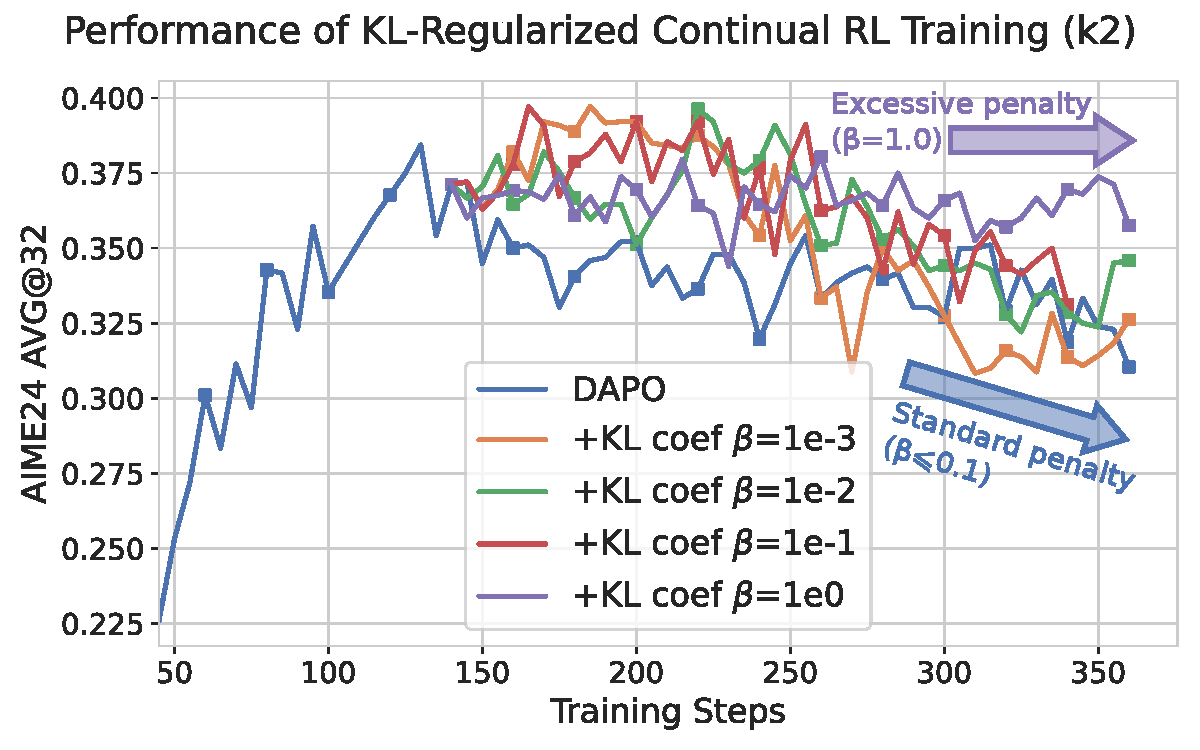
\includegraphics[width=\linewidth]{figs/k2_kl.pdf}
    \caption{\textbf{KL-regularized training performance (using \texttt{k2} estimation).}
    Consistent with \texttt{k3} results (Fig.~\ref{fig:kl_perf}), standard penalties ($\beta \le 0.1$: \textcolor{myorange}{1e-3}, \textcolor{mygreen}{1e-2}, \textcolor{myred}{1e-1}) merely delay validation collapse. The extreme setting (\textcolor{mypurple}{$\beta$ = 1.0}) enforces stability but induces stagnation, validating the stability-plasticity dilemma in KL-regularization.}
    \label{fig:kl_perf_k2}
\end{figure}

\begin{figure*}[t]
    \centering
    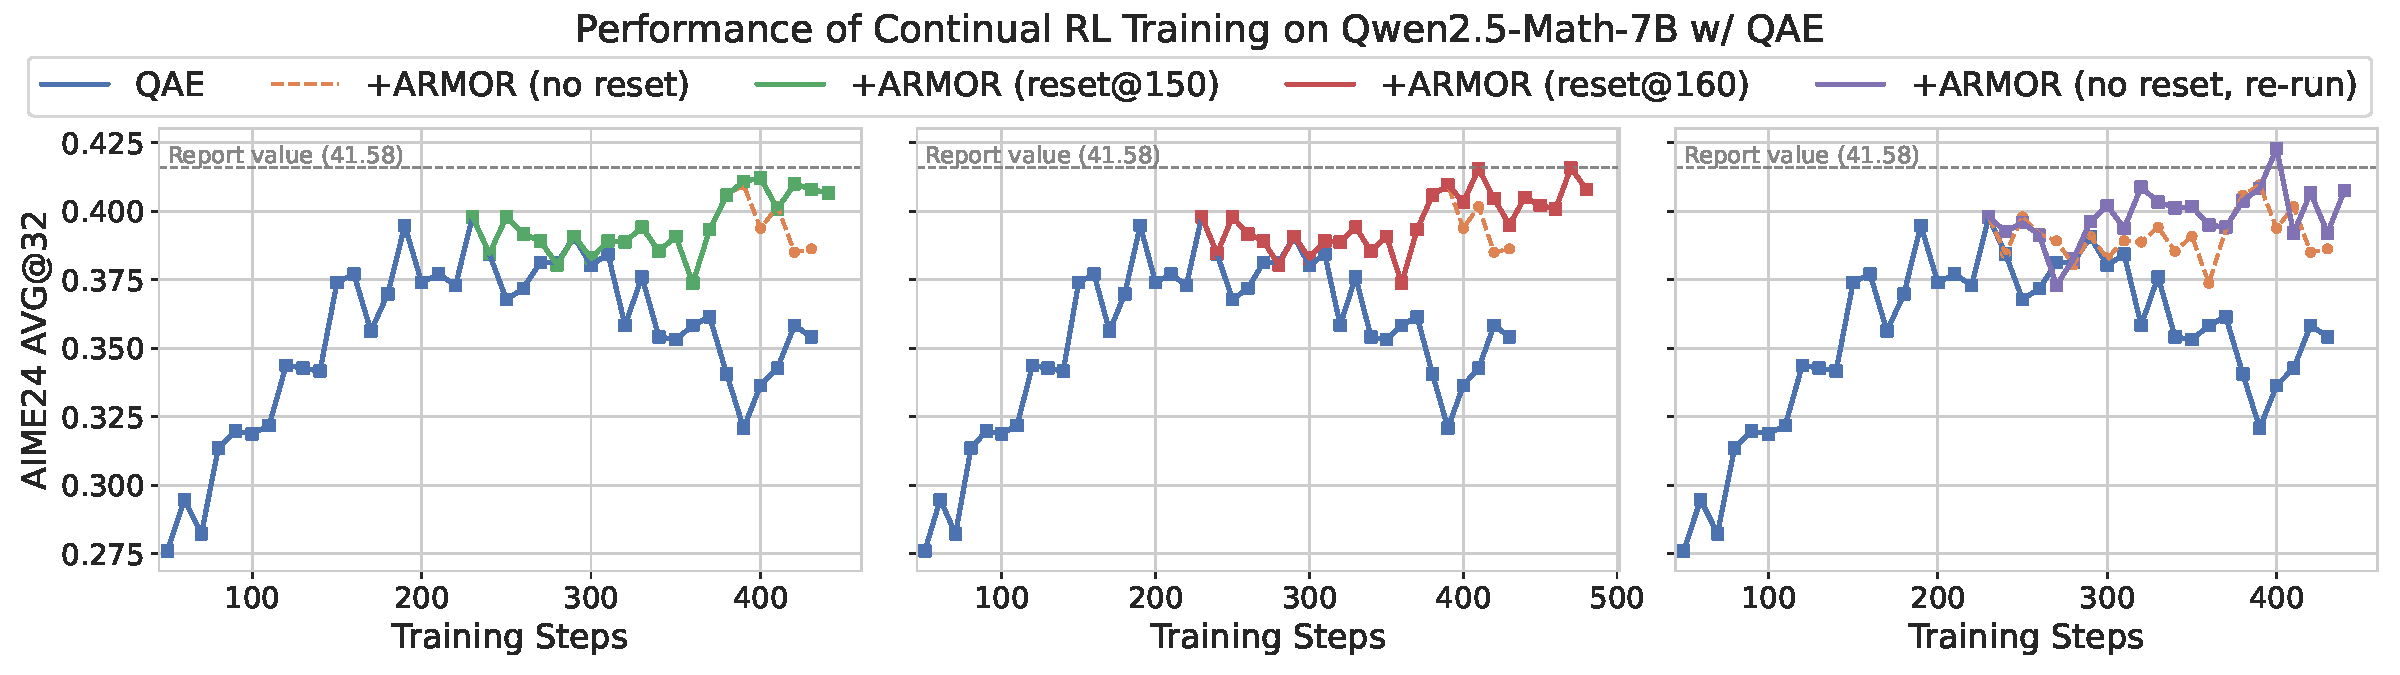
\includegraphics[width=\linewidth]{figs/qae.pdf}
    \caption{Hyperparameter robustness of ARMOR on QAE.
    We compare ARMOR variants against the \textcolor{myblue}{QAE baseline}.
    Across all settings---whether using \textcolor{myorange}{static anchors}, periodic resets after \textcolor{mygreen}{150 steps}, \textcolor{myred}{160 steps}, or \textcolor{mypurple}{a distinct re-run}---ARMOR consistently stabilizes training and maintains high performance.
    Notably, all variants approach or surpass the reported peak performance (AIME24 \texttt{avg@32=41.58}, indicated by the \textcolor{gray}{gray dashed line}).}
    \label{fig:qae}
\end{figure*}

\subsection{KL Regularization with \texttt{k2} Estimation}
In Section~\ref{sec:kl}, we analyzed continual training using the standard \texttt{k3} estimator for reverse KL.
To ensure our conclusions are robust to estimator choice, we extend this analysis using the \texttt{k2} estimator, which is shown to provide unbiased gradient estimation \citep{klpitfalls}.
As illustrated in Fig.~\ref{fig:kl_perf_k2}, the performance dynamics mirror those observed with \texttt{k3}: standard penalties ($\beta \le 0.1$) fail to prevent eventual collapse, whereas excessive penalties ($\beta=1.0$) secure stability only at the cost of stagnation.
This confirms that the stability-plasticity dilemma is intrinsic to the KL objective itself, rather than an artifact of the estimation method.

\subsection{Comparison with Teacher-Guided Two-Stage Training}\label{appendix:two_stage}

Beyond directly continuing RL from the best zero-RL checkpoint, another natural two-stage strategy is to use this checkpoint as a teacher policy for on-policy distillation.
We therefore compare ARMOR with OPD~\citep{agarwal2024policy} and MOPD~\citep{xiao2026mimo} under the same DAPO-trained reference policy.
As shown in Tab.~\ref{tab:two_stage}, OPD and MOPD provide stable teacher-guided training but only marginally improve over the reference checkpoint.
In contrast, ARMOR achieves substantially larger gains across both base models, indicating that explicitly targeting over-optimization is more effective than simply distilling from the zero-RL model.

\subsection{Hyperparameter Robustness}

While the main body of our paper focuses on ablations using DAPO + Qwen2.5-Math-7B, we further evaluate the robustness of ARMOR's hyperparameters across different algorithms and base models.

Firstly, we present a detailed comparison using the \textbf{QAE + Qwen2.5-Math-7B} setting.
Starting from the best QAE checkpoint (Step 230), we assess four variants of ARMOR to analyze the impact of reset frequency and training stochasticity. 
As illustrated in Fig.~\ref{fig:qae}, we compare:
\begin{enumerate}%[nosep]
    \item \textcolor{myorange}{ARMOR (no reset)}: We freeze the reference policy $\pi_\text{ref}$ throughout the training phase.
    \item \textcolor{mygreen}{ARMOR (reset@150)}: The reference policy is updated ($\pi_\text{ref}\leftarrow\pi_\theta$) every 150 steps during continual training.
    \item \textcolor{myred}{ARMOR (reset@160)}: The reference policy is updated every 160 steps.
    \item \textcolor{mypurple}{ARMOR (no reset, re-run)}: This is a reproducibility check on no-reset. To verify stability against the inherent randomness of RL training (e.g., rollout randomness), we conduct an independent re-run of the static anchor setting.
\end{enumerate}


\begin{figure*}[t]
    \centering
    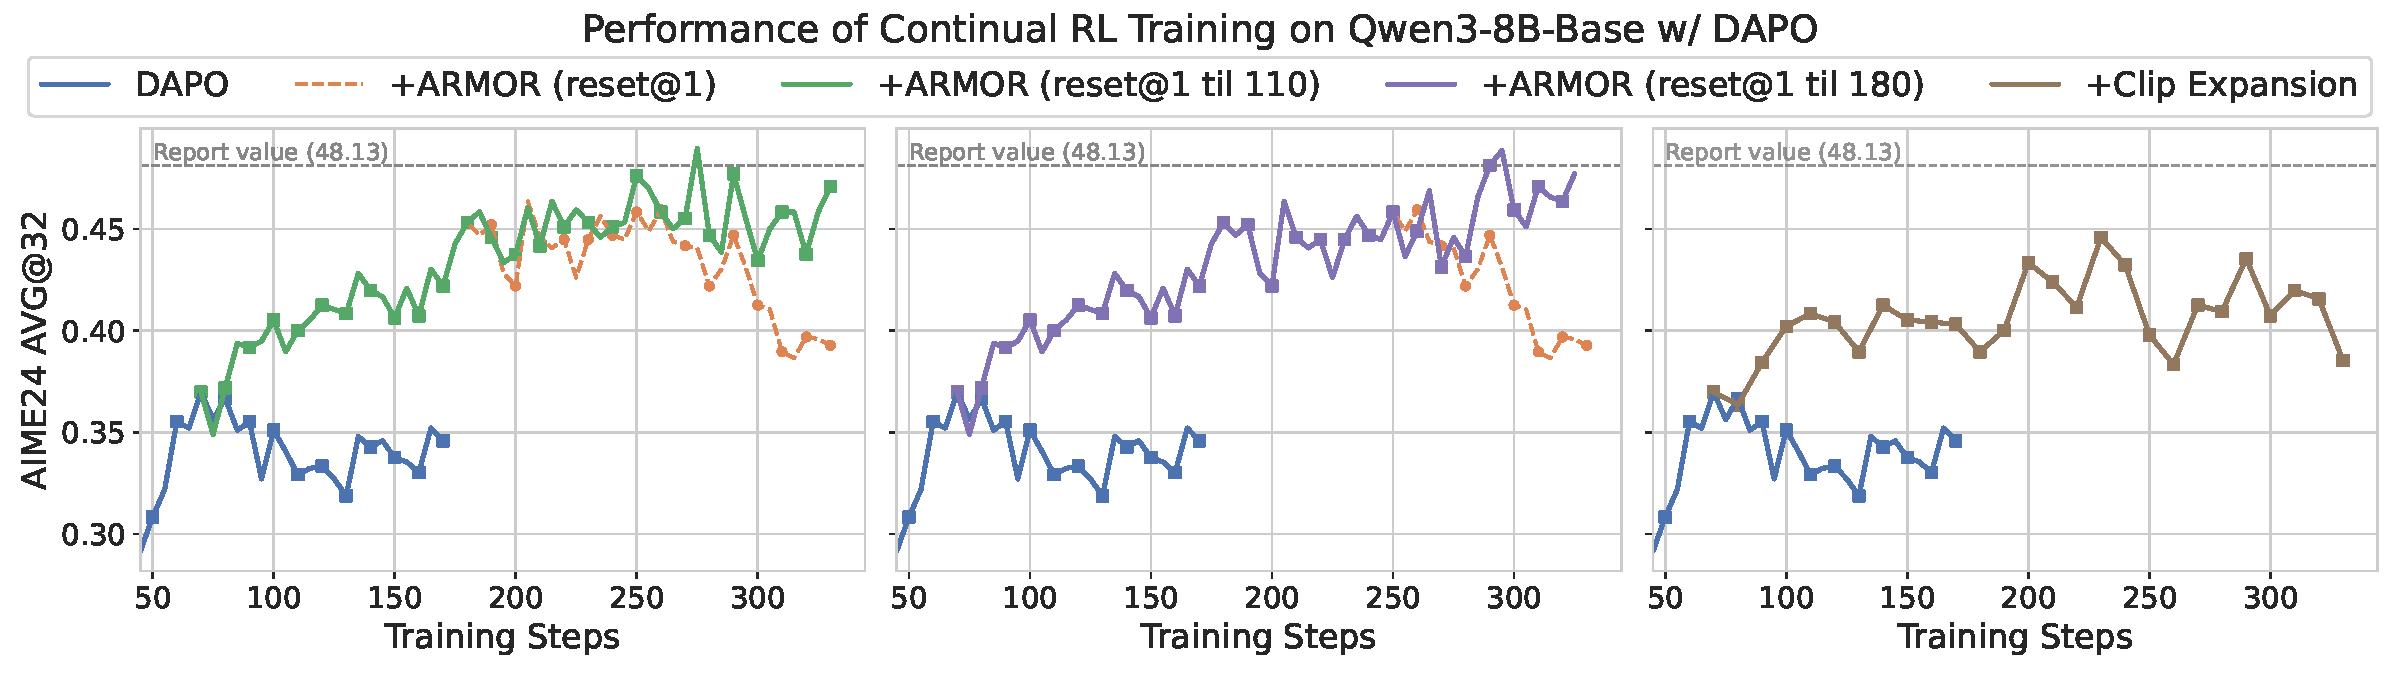
\includegraphics[width=\linewidth]{figs/qwen3.pdf}
    \caption{Ablation of Reset Strategy on Qwen3-8B-Base.
    Due to Qwen3's strong capability, continuous reference updates (\textcolor{myorange}{reset@1, \ie $\tau=1$}) enable rapid early gains but suffer from late-stage instability (orange dashed line).
    Our Hybrid Strategy (\textcolor{mygreen}{reset@1 til 110} and \textcolor{mypurple}{reset@1 til 180}) resolves this by freezing the anchor after an initial adaptation phase, both reaching the reported peak performance (AIME24 \texttt{avg@32=48.13}).
    In contrast, the \textcolor{mybrown}{Static Clip Expansion} baseline yields lower and more unstable performance, confirming that ARMOR's benefit stems from structure-aware regularization rather than simple clip relaxation.}
    \label{fig:qwen3}
\end{figure*}

The results in Fig.~\ref{fig:qae} demonstrate strong algorithmic robustness. 
While the \textcolor{myblue}{baseline QAE} suffers from performance degradation, all ARMOR variants successfully sustain the performance and approach or surpass the reported AIME24 value in Tab.~\ref{tab:main}, demonstrating that the gains are robust.

Next, we present a comparison using the \textbf{DAPO + Qwen3-8B-Base} setting.

Unlike the Qwen2.5-Math-7B model, Qwen3 is a strong base model with high intrinsic reasoning potential.
We hypothesize that in the continual training setting, such a model benefits from a more aggressive exploration space in the early stages, without being strictly tethered to a static reference.
To validate this, we compare the following strategies (Fig.~\ref{fig:qwen3}):

\begin{enumerate}%[nosep]
    \item \textcolor{myorange}{ARMOR (reset@1)} We reset the reference policy at every step. This maximizes the adaptivity of the trust region but minimizes the ``anchoring'' effect.
    \item \textcolor{mygreen}{ARMOR (reset@1 til 110)} and \textcolor{mypurple}{ARMOR (reset@1 til 180}): We adopt a two-stage schedule: updating the reference at every step ($\tau=1$) for the first $T$ steps (110 or 180) to facilitate rapid adaptation, then freezing the reference policy to secure stability.
    \item \textcolor{mybrown}{Clip Expansion}: To verify that ARMOR's gain is not merely due to a wider clip range, we test a baseline using standard DAPO with a manually expanded clip range matching ARMOR's theoretical boundary (as detailed in Sec.~\ref{sec:mix_ablation}).
\end{enumerate}

\textbf{Analysis.}
The results reveal three key insights:
\textit{(1) Necessity of Anchors}: Continuous updates ($\tau=1$) accelerate early adaptation but eventually degrade due to the loss of anchor stabilization, confirming the need for a fixed reference in the late stage.
\textit{(2) Effectiveness and Robustness}: The hybrid strategy secures the best of both worlds: rapid early exploration and sustained stability. Notably, both freeze timings (180/250 steps) reach the reported ceiling, demonstrating ARMOR's robustness to the specific schedule.
\textit{(3) Superiority over Simple Relaxation}: The instability of Static Clip Expansion confirms that ARMOR's benefit derives from principled, direction-aware regularization rather than a generic relaxation of constraints.


% \begin{figure}
%     \centering
%     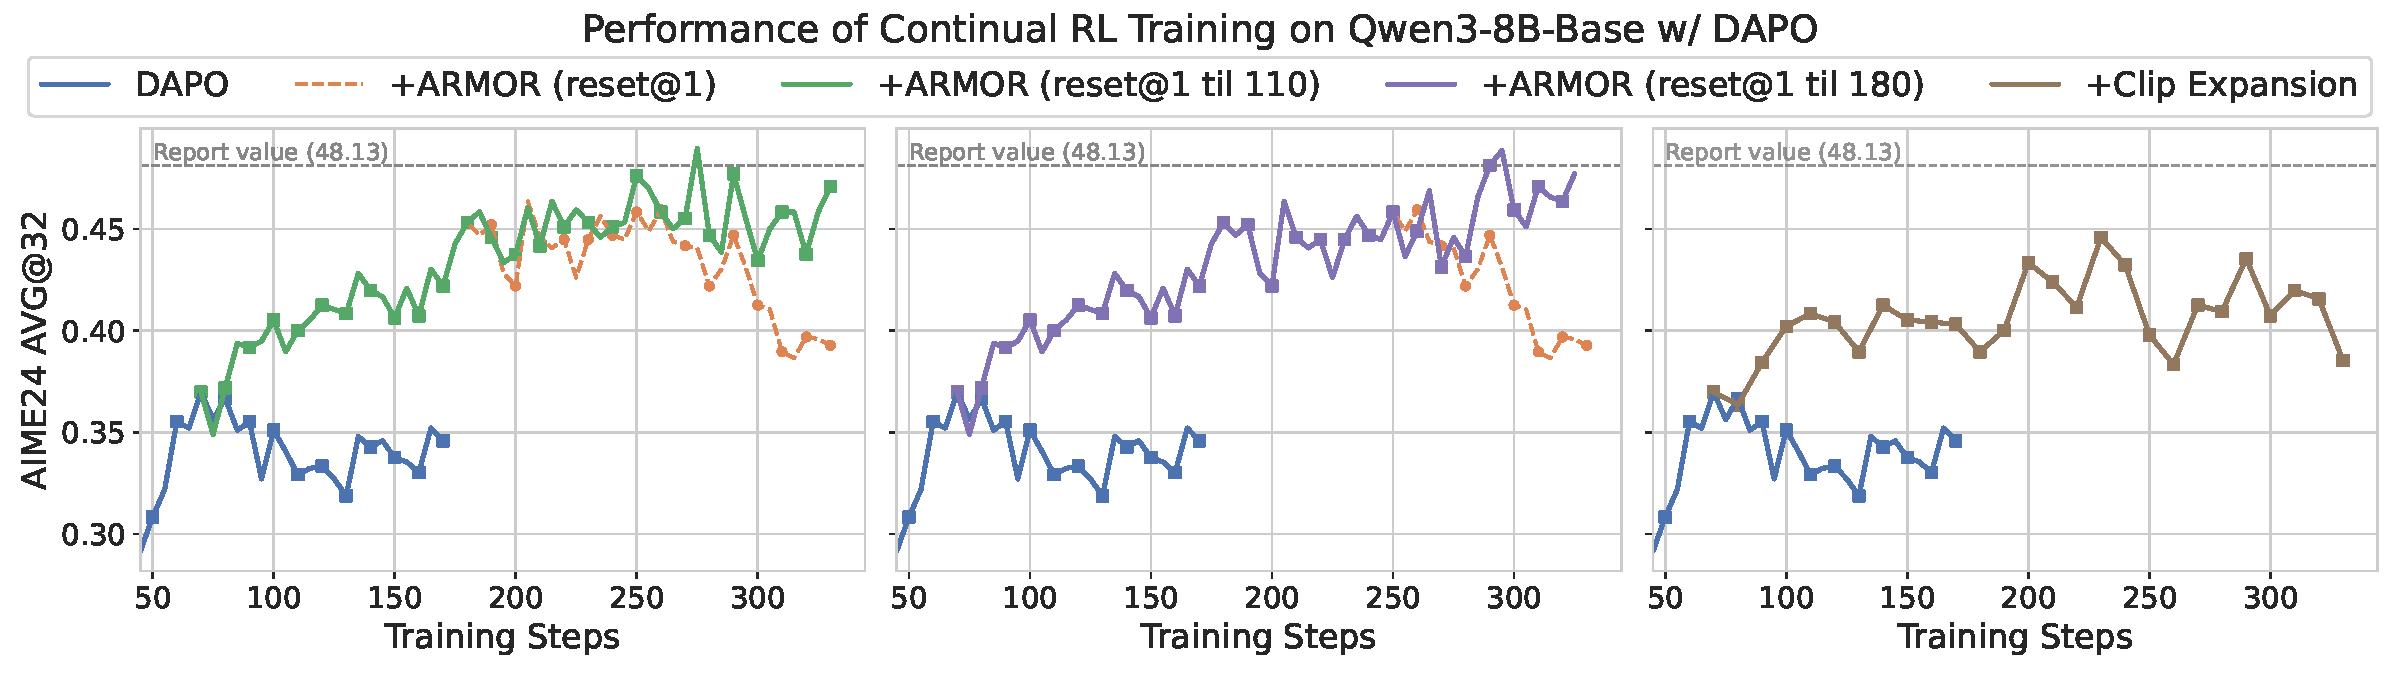
\includegraphics[width=0.9\linewidth]{figs/qwen3.pdf}
%     \caption{Qwen3}
%     \label{fig:qwen3}
% \end{figure}
\section{Potential Risks}
This paper is mainly concerned with algorithmic advances in reinforcement learning for large language models. The proposed method does not introduce new application scenarios, datasets, deployment settings, or model capabilities that would create risks beyond those generally associated with LLM post-training. Therefore, we do not foresee specific potential risks unique to this work, while acknowledging that general LLM-related risks such as misuse, hallucination, and biased generation remain relevant.


\section{Artifacts and Licenses}
The artifacts used in this work, including code, datasets, and model checkpoints, are listed below together with their corresponding licenses. We use these artifacts in accordance with their intended research use and license terms.

\begin{itemize}[left=0em,topsep=0pt,itemsep=0pt]
    \item DAPO's training recipe, including the released code, training scripts, and training data: Apache 2.0 License.
    \item AIME datasets: Apache 2.0 License. These datasets are used only for evaluation.
    \item AMC dataset: Apache 2.0 License. The dataset is used only for evaluation.
    \item GPQA dataset: Creative Commons Attribution 4.0 International (CC BY 4.0) License.
    \item MMLU-Pro dataset: MIT License.
    \item Qwen-2.5-Math model: Apache 2.0 License.
    \item Qwen-3-8B-Base model: Apache 2.0 License.
\end{itemize}

We do not introduce new datasets containing private, sensitive, or personally identifiable information. All external artifacts are publicly available, and our use of them is limited to algorithm development and benchmark evaluation.


\section{The use of LLMs}
We utilize LLMs only to polish some of the language of this paper.
All content was originally drafted by the authors. 
The use of LLMs was restricted to refining some pre-existing text, and any suggested modifications were reviewed by the authors to confirm their accuracy and alignment with the original meaning.